\documentclass[10pt]{article} % For LaTeX2e
\usepackage{tmlr}
% If accepted, instead use the following line for the camera-ready submission:
%\usepackage[accepted]{tmlr}
% To de-anonymize and remove mentions to TMLR (for example for posting to preprint servers), instead use the following:
%\usepackage[preprint]{tmlr}

% Optional math commands from https://github.com/goodfeli/dlbook_notation.
%%%%% NEW MATH DEFINITIONS %%%%%

\usepackage{amsmath,amsfonts,bm}

% Mark sections of captions for referring to divisions of figures
\newcommand{\figleft}{{\em (Left)}}
\newcommand{\figcenter}{{\em (Center)}}
\newcommand{\figright}{{\em (Right)}}
\newcommand{\figtop}{{\em (Top)}}
\newcommand{\figbottom}{{\em (Bottom)}}
\newcommand{\captiona}{{\em (a)}}
\newcommand{\captionb}{{\em (b)}}
\newcommand{\captionc}{{\em (c)}}
\newcommand{\captiond}{{\em (d)}}

% Highlight a newly defined term
\newcommand{\newterm}[1]{{\bf #1}}


% Figure reference, lower-case.
\def\figref#1{figure~\ref{#1}}
% Figure reference, capital. For start of sentence
\def\Figref#1{Figure~\ref{#1}}
\def\twofigref#1#2{figures \ref{#1} and \ref{#2}}
\def\quadfigref#1#2#3#4{figures \ref{#1}, \ref{#2}, \ref{#3} and \ref{#4}}
% Section reference, lower-case.
\def\secref#1{section~\ref{#1}}
% Section reference, capital.
\def\Secref#1{Section~\ref{#1}}
% Reference to two sections.
\def\twosecrefs#1#2{sections \ref{#1} and \ref{#2}}
% Reference to three sections.
\def\secrefs#1#2#3{sections \ref{#1}, \ref{#2} and \ref{#3}}
% Reference to an equation, lower-case.
\def\eqref#1{equation~\ref{#1}}
% Reference to an equation, upper case
\def\Eqref#1{Equation~\ref{#1}}
% A raw reference to an equation---avoid using if possible
\def\plaineqref#1{\ref{#1}}
% Reference to a chapter, lower-case.
\def\chapref#1{chapter~\ref{#1}}
% Reference to an equation, upper case.
\def\Chapref#1{Chapter~\ref{#1}}
% Reference to a range of chapters
\def\rangechapref#1#2{chapters\ref{#1}--\ref{#2}}
% Reference to an algorithm, lower-case.
\def\algref#1{algorithm~\ref{#1}}
% Reference to an algorithm, upper case.
\def\Algref#1{Algorithm~\ref{#1}}
\def\twoalgref#1#2{algorithms \ref{#1} and \ref{#2}}
\def\Twoalgref#1#2{Algorithms \ref{#1} and \ref{#2}}
% Reference to a part, lower case
\def\partref#1{part~\ref{#1}}
% Reference to a part, upper case
\def\Partref#1{Part~\ref{#1}}
\def\twopartref#1#2{parts \ref{#1} and \ref{#2}}

\def\ceil#1{\lceil #1 \rceil}
\def\floor#1{\lfloor #1 \rfloor}
\def\1{\bm{1}}
\newcommand{\train}{\mathcal{D}}
\newcommand{\valid}{\mathcal{D_{\mathrm{valid}}}}
\newcommand{\test}{\mathcal{D_{\mathrm{test}}}}

\def\eps{{\epsilon}}


% Random variables
\def\reta{{\textnormal{$\eta$}}}
\def\ra{{\textnormal{a}}}
\def\rb{{\textnormal{b}}}
\def\rc{{\textnormal{c}}}
\def\rd{{\textnormal{d}}}
\def\re{{\textnormal{e}}}
\def\rf{{\textnormal{f}}}
\def\rg{{\textnormal{g}}}
\def\rh{{\textnormal{h}}}
\def\ri{{\textnormal{i}}}
\def\rj{{\textnormal{j}}}
\def\rk{{\textnormal{k}}}
\def\rl{{\textnormal{l}}}
% rm is already a command, just don't name any random variables m
\def\rn{{\textnormal{n}}}
\def\ro{{\textnormal{o}}}
\def\rp{{\textnormal{p}}}
\def\rq{{\textnormal{q}}}
\def\rr{{\textnormal{r}}}
\def\rs{{\textnormal{s}}}
\def\rt{{\textnormal{t}}}
\def\ru{{\textnormal{u}}}
\def\rv{{\textnormal{v}}}
\def\rw{{\textnormal{w}}}
\def\rx{{\textnormal{x}}}
\def\ry{{\textnormal{y}}}
\def\rz{{\textnormal{z}}}

% Random vectors
\def\rvepsilon{{\mathbf{\epsilon}}}
\def\rvtheta{{\mathbf{\theta}}}
\def\rva{{\mathbf{a}}}
\def\rvb{{\mathbf{b}}}
\def\rvc{{\mathbf{c}}}
\def\rvd{{\mathbf{d}}}
\def\rve{{\mathbf{e}}}
\def\rvf{{\mathbf{f}}}
\def\rvg{{\mathbf{g}}}
\def\rvh{{\mathbf{h}}}
\def\rvu{{\mathbf{i}}}
\def\rvj{{\mathbf{j}}}
\def\rvk{{\mathbf{k}}}
\def\rvl{{\mathbf{l}}}
\def\rvm{{\mathbf{m}}}
\def\rvn{{\mathbf{n}}}
\def\rvo{{\mathbf{o}}}
\def\rvp{{\mathbf{p}}}
\def\rvq{{\mathbf{q}}}
\def\rvr{{\mathbf{r}}}
\def\rvs{{\mathbf{s}}}
\def\rvt{{\mathbf{t}}}
\def\rvu{{\mathbf{u}}}
\def\rvv{{\mathbf{v}}}
\def\rvw{{\mathbf{w}}}
\def\rvx{{\mathbf{x}}}
\def\rvy{{\mathbf{y}}}
\def\rvz{{\mathbf{z}}}

% Elements of random vectors
\def\erva{{\textnormal{a}}}
\def\ervb{{\textnormal{b}}}
\def\ervc{{\textnormal{c}}}
\def\ervd{{\textnormal{d}}}
\def\erve{{\textnormal{e}}}
\def\ervf{{\textnormal{f}}}
\def\ervg{{\textnormal{g}}}
\def\ervh{{\textnormal{h}}}
\def\ervi{{\textnormal{i}}}
\def\ervj{{\textnormal{j}}}
\def\ervk{{\textnormal{k}}}
\def\ervl{{\textnormal{l}}}
\def\ervm{{\textnormal{m}}}
\def\ervn{{\textnormal{n}}}
\def\ervo{{\textnormal{o}}}
\def\ervp{{\textnormal{p}}}
\def\ervq{{\textnormal{q}}}
\def\ervr{{\textnormal{r}}}
\def\ervs{{\textnormal{s}}}
\def\ervt{{\textnormal{t}}}
\def\ervu{{\textnormal{u}}}
\def\ervv{{\textnormal{v}}}
\def\ervw{{\textnormal{w}}}
\def\ervx{{\textnormal{x}}}
\def\ervy{{\textnormal{y}}}
\def\ervz{{\textnormal{z}}}

% Random matrices
\def\rmA{{\mathbf{A}}}
\def\rmB{{\mathbf{B}}}
\def\rmC{{\mathbf{C}}}
\def\rmD{{\mathbf{D}}}
\def\rmE{{\mathbf{E}}}
\def\rmF{{\mathbf{F}}}
\def\rmG{{\mathbf{G}}}
\def\rmH{{\mathbf{H}}}
\def\rmI{{\mathbf{I}}}
\def\rmJ{{\mathbf{J}}}
\def\rmK{{\mathbf{K}}}
\def\rmL{{\mathbf{L}}}
\def\rmM{{\mathbf{M}}}
\def\rmN{{\mathbf{N}}}
\def\rmO{{\mathbf{O}}}
\def\rmP{{\mathbf{P}}}
\def\rmQ{{\mathbf{Q}}}
\def\rmR{{\mathbf{R}}}
\def\rmS{{\mathbf{S}}}
\def\rmT{{\mathbf{T}}}
\def\rmU{{\mathbf{U}}}
\def\rmV{{\mathbf{V}}}
\def\rmW{{\mathbf{W}}}
\def\rmX{{\mathbf{X}}}
\def\rmY{{\mathbf{Y}}}
\def\rmZ{{\mathbf{Z}}}

% Elements of random matrices
\def\ermA{{\textnormal{A}}}
\def\ermB{{\textnormal{B}}}
\def\ermC{{\textnormal{C}}}
\def\ermD{{\textnormal{D}}}
\def\ermE{{\textnormal{E}}}
\def\ermF{{\textnormal{F}}}
\def\ermG{{\textnormal{G}}}
\def\ermH{{\textnormal{H}}}
\def\ermI{{\textnormal{I}}}
\def\ermJ{{\textnormal{J}}}
\def\ermK{{\textnormal{K}}}
\def\ermL{{\textnormal{L}}}
\def\ermM{{\textnormal{M}}}
\def\ermN{{\textnormal{N}}}
\def\ermO{{\textnormal{O}}}
\def\ermP{{\textnormal{P}}}
\def\ermQ{{\textnormal{Q}}}
\def\ermR{{\textnormal{R}}}
\def\ermS{{\textnormal{S}}}
\def\ermT{{\textnormal{T}}}
\def\ermU{{\textnormal{U}}}
\def\ermV{{\textnormal{V}}}
\def\ermW{{\textnormal{W}}}
\def\ermX{{\textnormal{X}}}
\def\ermY{{\textnormal{Y}}}
\def\ermZ{{\textnormal{Z}}}

% Vectors
\def\vzero{{\bm{0}}}
\def\vone{{\bm{1}}}
\def\vmu{{\bm{\mu}}}
\def\vtheta{{\bm{\theta}}}
\def\va{{\bm{a}}}
\def\vb{{\bm{b}}}
\def\vc{{\bm{c}}}
\def\vd{{\bm{d}}}
\def\ve{{\bm{e}}}
\def\vf{{\bm{f}}}
\def\vg{{\bm{g}}}
\def\vh{{\bm{h}}}
\def\vi{{\bm{i}}}
\def\vj{{\bm{j}}}
\def\vk{{\bm{k}}}
\def\vl{{\bm{l}}}
\def\vm{{\bm{m}}}
\def\vn{{\bm{n}}}
\def\vo{{\bm{o}}}
\def\vp{{\bm{p}}}
\def\vq{{\bm{q}}}
\def\vr{{\bm{r}}}
\def\vs{{\bm{s}}}
\def\vt{{\bm{t}}}
\def\vu{{\bm{u}}}
\def\vv{{\bm{v}}}
\def\vw{{\bm{w}}}
\def\vx{{\bm{x}}}
\def\vy{{\bm{y}}}
\def\vz{{\bm{z}}}

% Elements of vectors
\def\evalpha{{\alpha}}
\def\evbeta{{\beta}}
\def\evepsilon{{\epsilon}}
\def\evlambda{{\lambda}}
\def\evomega{{\omega}}
\def\evmu{{\mu}}
\def\evpsi{{\psi}}
\def\evsigma{{\sigma}}
\def\evtheta{{\theta}}
\def\eva{{a}}
\def\evb{{b}}
\def\evc{{c}}
\def\evd{{d}}
\def\eve{{e}}
\def\evf{{f}}
\def\evg{{g}}
\def\evh{{h}}
\def\evi{{i}}
\def\evj{{j}}
\def\evk{{k}}
\def\evl{{l}}
\def\evm{{m}}
\def\evn{{n}}
\def\evo{{o}}
\def\evp{{p}}
\def\evq{{q}}
\def\evr{{r}}
\def\evs{{s}}
\def\evt{{t}}
\def\evu{{u}}
\def\evv{{v}}
\def\evw{{w}}
\def\evx{{x}}
\def\evy{{y}}
\def\evz{{z}}

% Matrix
\def\mA{{\bm{A}}}
\def\mB{{\bm{B}}}
\def\mC{{\bm{C}}}
\def\mD{{\bm{D}}}
\def\mE{{\bm{E}}}
\def\mF{{\bm{F}}}
\def\mG{{\bm{G}}}
\def\mH{{\bm{H}}}
\def\mI{{\bm{I}}}
\def\mJ{{\bm{J}}}
\def\mK{{\bm{K}}}
\def\mL{{\bm{L}}}
\def\mM{{\bm{M}}}
\def\mN{{\bm{N}}}
\def\mO{{\bm{O}}}
\def\mP{{\bm{P}}}
\def\mQ{{\bm{Q}}}
\def\mR{{\bm{R}}}
\def\mS{{\bm{S}}}
\def\mT{{\bm{T}}}
\def\mU{{\bm{U}}}
\def\mV{{\bm{V}}}
\def\mW{{\bm{W}}}
\def\mX{{\bm{X}}}
\def\mY{{\bm{Y}}}
\def\mZ{{\bm{Z}}}
\def\mBeta{{\bm{\beta}}}
\def\mPhi{{\bm{\Phi}}}
\def\mLambda{{\bm{\Lambda}}}
\def\mSigma{{\bm{\Sigma}}}

% Tensor
\DeclareMathAlphabet{\mathsfit}{\encodingdefault}{\sfdefault}{m}{sl}
\SetMathAlphabet{\mathsfit}{bold}{\encodingdefault}{\sfdefault}{bx}{n}
\newcommand{\tens}[1]{\bm{\mathsfit{#1}}}
\def\tA{{\tens{A}}}
\def\tB{{\tens{B}}}
\def\tC{{\tens{C}}}
\def\tD{{\tens{D}}}
\def\tE{{\tens{E}}}
\def\tF{{\tens{F}}}
\def\tG{{\tens{G}}}
\def\tH{{\tens{H}}}
\def\tI{{\tens{I}}}
\def\tJ{{\tens{J}}}
\def\tK{{\tens{K}}}
\def\tL{{\tens{L}}}
\def\tM{{\tens{M}}}
\def\tN{{\tens{N}}}
\def\tO{{\tens{O}}}
\def\tP{{\tens{P}}}
\def\tQ{{\tens{Q}}}
\def\tR{{\tens{R}}}
\def\tS{{\tens{S}}}
\def\tT{{\tens{T}}}
\def\tU{{\tens{U}}}
\def\tV{{\tens{V}}}
\def\tW{{\tens{W}}}
\def\tX{{\tens{X}}}
\def\tY{{\tens{Y}}}
\def\tZ{{\tens{Z}}}


% Graph
\def\gA{{\mathcal{A}}}
\def\gB{{\mathcal{B}}}
\def\gC{{\mathcal{C}}}
\def\gD{{\mathcal{D}}}
\def\gE{{\mathcal{E}}}
\def\gF{{\mathcal{F}}}
\def\gG{{\mathcal{G}}}
\def\gH{{\mathcal{H}}}
\def\gI{{\mathcal{I}}}
\def\gJ{{\mathcal{J}}}
\def\gK{{\mathcal{K}}}
\def\gL{{\mathcal{L}}}
\def\gM{{\mathcal{M}}}
\def\gN{{\mathcal{N}}}
\def\gO{{\mathcal{O}}}
\def\gP{{\mathcal{P}}}
\def\gQ{{\mathcal{Q}}}
\def\gR{{\mathcal{R}}}
\def\gS{{\mathcal{S}}}
\def\gT{{\mathcal{T}}}
\def\gU{{\mathcal{U}}}
\def\gV{{\mathcal{V}}}
\def\gW{{\mathcal{W}}}
\def\gX{{\mathcal{X}}}
\def\gY{{\mathcal{Y}}}
\def\gZ{{\mathcal{Z}}}

% Sets
\def\sA{{\mathbb{A}}}
\def\sB{{\mathbb{B}}}
\def\sC{{\mathbb{C}}}
\def\sD{{\mathbb{D}}}
% Don't use a set called E, because this would be the same as our symbol
% for expectation.
\def\sF{{\mathbb{F}}}
\def\sG{{\mathbb{G}}}
\def\sH{{\mathbb{H}}}
\def\sI{{\mathbb{I}}}
\def\sJ{{\mathbb{J}}}
\def\sK{{\mathbb{K}}}
\def\sL{{\mathbb{L}}}
\def\sM{{\mathbb{M}}}
\def\sN{{\mathbb{N}}}
\def\sO{{\mathbb{O}}}
\def\sP{{\mathbb{P}}}
\def\sQ{{\mathbb{Q}}}
\def\sR{{\mathbb{R}}}
\def\sS{{\mathbb{S}}}
\def\sT{{\mathbb{T}}}
\def\sU{{\mathbb{U}}}
\def\sV{{\mathbb{V}}}
\def\sW{{\mathbb{W}}}
\def\sX{{\mathbb{X}}}
\def\sY{{\mathbb{Y}}}
\def\sZ{{\mathbb{Z}}}

% Entries of a matrix
\def\emLambda{{\Lambda}}
\def\emA{{A}}
\def\emB{{B}}
\def\emC{{C}}
\def\emD{{D}}
\def\emE{{E}}
\def\emF{{F}}
\def\emG{{G}}
\def\emH{{H}}
\def\emI{{I}}
\def\emJ{{J}}
\def\emK{{K}}
\def\emL{{L}}
\def\emM{{M}}
\def\emN{{N}}
\def\emO{{O}}
\def\emP{{P}}
\def\emQ{{Q}}
\def\emR{{R}}
\def\emS{{S}}
\def\emT{{T}}
\def\emU{{U}}
\def\emV{{V}}
\def\emW{{W}}
\def\emX{{X}}
\def\emY{{Y}}
\def\emZ{{Z}}
\def\emSigma{{\Sigma}}

% entries of a tensor
% Same font as tensor, without \bm wrapper
\newcommand{\etens}[1]{\mathsfit{#1}}
\def\etLambda{{\etens{\Lambda}}}
\def\etA{{\etens{A}}}
\def\etB{{\etens{B}}}
\def\etC{{\etens{C}}}
\def\etD{{\etens{D}}}
\def\etE{{\etens{E}}}
\def\etF{{\etens{F}}}
\def\etG{{\etens{G}}}
\def\etH{{\etens{H}}}
\def\etI{{\etens{I}}}
\def\etJ{{\etens{J}}}
\def\etK{{\etens{K}}}
\def\etL{{\etens{L}}}
\def\etM{{\etens{M}}}
\def\etN{{\etens{N}}}
\def\etO{{\etens{O}}}
\def\etP{{\etens{P}}}
\def\etQ{{\etens{Q}}}
\def\etR{{\etens{R}}}
\def\etS{{\etens{S}}}
\def\etT{{\etens{T}}}
\def\etU{{\etens{U}}}
\def\etV{{\etens{V}}}
\def\etW{{\etens{W}}}
\def\etX{{\etens{X}}}
\def\etY{{\etens{Y}}}
\def\etZ{{\etens{Z}}}

% The true underlying data generating distribution
\newcommand{\pdata}{p_{\rm{data}}}
% The empirical distribution defined by the training set
\newcommand{\ptrain}{\hat{p}_{\rm{data}}}
\newcommand{\Ptrain}{\hat{P}_{\rm{data}}}
% The model distribution
\newcommand{\pmodel}{p_{\rm{model}}}
\newcommand{\Pmodel}{P_{\rm{model}}}
\newcommand{\ptildemodel}{\tilde{p}_{\rm{model}}}
% Stochastic autoencoder distributions
\newcommand{\pencode}{p_{\rm{encoder}}}
\newcommand{\pdecode}{p_{\rm{decoder}}}
\newcommand{\precons}{p_{\rm{reconstruct}}}

\newcommand{\laplace}{\mathrm{Laplace}} % Laplace distribution

\newcommand{\E}{\mathbb{E}}
\newcommand{\Ls}{\mathcal{L}}
\newcommand{\R}{\mathbb{R}}
\newcommand{\emp}{\tilde{p}}
\newcommand{\lr}{\alpha}
\newcommand{\reg}{\lambda}
\newcommand{\rect}{\mathrm{rectifier}}
\newcommand{\softmax}{\mathrm{softmax}}
\newcommand{\sigmoid}{\sigma}
\newcommand{\softplus}{\zeta}
\newcommand{\KL}{D_{\mathrm{KL}}}
\newcommand{\Var}{\mathrm{Var}}
\newcommand{\standarderror}{\mathrm{SE}}
\newcommand{\Cov}{\mathrm{Cov}}
% Wolfram Mathworld says $L^2$ is for function spaces and $\ell^2$ is for vectors
% But then they seem to use $L^2$ for vectors throughout the site, and so does
% wikipedia.
\newcommand{\normlzero}{L^0}
\newcommand{\normlone}{L^1}
\newcommand{\normltwo}{L^2}
\newcommand{\normlp}{L^p}
\newcommand{\normmax}{L^\infty}

\newcommand{\parents}{Pa} % See usage in notation.tex. Chosen to match Daphne's book.

\DeclareMathOperator*{\argmax}{arg\,max}
\DeclareMathOperator*{\argmin}{arg\,min}

\DeclareMathOperator{\sign}{sign}
\DeclareMathOperator{\Tr}{Tr}
\let\ab\allowbreak


\usepackage{hyperref}
\usepackage{url}
\usepackage{graphicx}
\usepackage{booktabs}
\usepackage{amssymb}

% notation used throughout
\newcommand{\dW}{\Delta W}
\newcommand{\thresholdrank}{\rho_{0.01}}
\newcommand{\energyrank}{k_{0.9}}
\newcommand{\entropyrank}{\mathrm{eRank}}
\newcommand{\stablerank}{\mathrm{sr}}

\title{Rank Measures of Fine-Tuning Updates\\Need a Noise Baseline}

% Authors must not appear in the submitted version. They should be hidden
% as long as the tmlr package is used without the [accepted] or [preprint] options.
% Non-anonymous submissions will be rejected without review.

\author{\name Muhammad Usman Altaf \email email@example.com \\
      \addr Independent Researcher}
% TODO before the preprint: real email, and affiliation if not independent

\def\month{MM}  % Insert correct month for camera-ready version
\def\year{YYYY} % Insert correct year for camera-ready version
\def\openreview{\url{https://openreview.net/forum?id=XXXX}} % Insert correct link to OpenReview for camera-ready version


\begin{document}


\maketitle

\begin{abstract}
Claims about what fine-tuning does to a language model's weights often rest on
the rank of the update $\dW = W_{\text{after}} - W_{\text{before}}$. We measure
four rank measures on real updates and on random matrices of the same shape.
Three measures in common use, the number of singular values above
$0.01\,\sigma_1$, the rank needed for 90\% of the energy, and the entropy
effective rank, put real updates only 0.4--31\% below the noise value, so that
read on their own they describe the updates as close to full rank. Stable rank,
$\|\dW\|_F^2/\|\dW\|_2^2$, puts the same updates 1.6--9$\times$ below noise.
All four detect structure; only stable rank makes its size visible. We show
this on full SFT, DPO and token-matched non-alignment fine-tunes of
Qwen2.5-0.5B and SmolLM2-360M, with seed repeats and layer-bootstrap
intervals, and on seven publicly released base/instruct pairs from 135M to 8B
parameters. The updates combine a few dominant directions with a long tail
that holds most of the energy, and they are at least as concentrated as the
pretrained weights they are added to. The concentration is not specific to alignment:
fine-tuning on Wikipedia text or Python code is as concentrated as instruction
tuning. As a case study we revisit Timber, which cites an unchanged entropy
effective rank between base and instruct weights as evidence that
post-training is superficial. A random perturbation of the same norm leaves
the effective rank just as unchanged. Timber's eRank cutoff for editing $\dW$
leaves 99\% of the update's energy untouched; a stable-rank cutoff that scales
53 times more of it gives the same GSM8K pass@$k$, and removing that tail
outright costs 4 points of pass@1.
\end{abstract}

\section{Introduction}
\label{sec:intro}

A recurring question about post-training is whether it teaches a model
anything or only selects a style it already had. The superficial alignment
hypothesis \citep{zhou2023lima} takes the second view, and output-level
evidence such as in-context alignment of base models \citep{lin2024urial}
supports it. A natural place to look for weight-level evidence is the update
itself, $\dW = W_{\text{after}} - W_{\text{before}}$: if alignment only picks
a style, perhaps $\dW$ should be small and structured, ideally low rank.

That question has to be answered with some measure of rank, and full-rank
dense matrices make the choice of measure matter. Three measures appear in
recent work: counting singular values above a fraction of the largest,
counting how many are needed to hold most of the energy
\citep{biderman2024lora}, and the entropy effective rank of
\citet{roy2007effective}, used by \citet{wu2025timber} to argue that
post-training is superficial. All three summarize the spectrum by how many
directions it spans. None of these uses compares the number against what a
matrix with no structure at all would give.

We set out to measure the rank of SFT and DPO updates on a small model and ran
into exactly this problem. By the threshold count, our SFT update was at 99.1\%
of full rank and the difference between two random initializations was at
99.6\%. Read at face value, that says the update looks like noise. Stable rank
\citep{rudelson2007sampling} on the same spectra says the opposite: the update
is three times more concentrated than the random pair, and its top direction
carries eight times the share of energy.

This paper is about that gap. Our contributions are:

\begin{itemize}
  \item \textbf{A noise baseline for every matrix.} We compare four rank
  measures on real updates against random matrices of the same shape and show
  that the threshold count, the 90\%-energy rank and the entropy effective
  rank all land within a few percent of the noise value, while stable rank
  separates real updates from noise by 1.6--9$\times$
  (\S\ref{sec:metrics}). The two readings are not in conflict: updates have a
  noise-like tail and a few dominant directions, and the measures weight these
  differently (\S\ref{sec:headtail}).
  \item \textbf{Controls that separate fine-tuning from alignment.}
  Token-matched fine-tunes on wikitext and Python code, with second seeds and
  paired layer-bootstrap intervals, are as concentrated as SFT on two model
  families (\S\ref{sec:controls}). Concentration of $\dW$ is a property of
  fine-tuning, not evidence about alignment.
  \item \textbf{Released models up to 8B.} The same pattern holds for seven
  official base/instruct pairs from 135M to 8B parameters (\S\ref{sec:released}).
  \item \textbf{A case study of Timber.} We reproduce the entropy effective
  rank measurement of \citet{wu2025timber} on two of its model pairs and show
  that its evidence for superficiality, an unchanged eRank of each weight
  matrix, is also produced by a random perturbation of the same norm. Its
  eRank cutoff for editing $\dW$ is not special: a cutoff that edits about
  40$\times$ more of the update gives the same GSM8K pass@$k$, and both effects
  are within a point of zero on the full test set (\S\ref{sec:timber}).
\end{itemize}

The training runs use a single 6\,GB GPU, so our own fine-tunes are small
(0.36B and 0.5B parameters, about two million tokens each). The measurement
results do not depend on training, and we check them on released models up to
8B. We report behavioural results from the same runs (LoRA rank sweep, DPO,
evals) in \S\ref{sec:behavior}, mostly as context.

\section{Measuring the rank of an update}
\label{sec:background}

Let $\dW \in \R^{m\times n}$ be the update to one weight matrix,
$r = \min(m,n)$, and $\sigma_1 \geq \dots \geq \sigma_r$ its singular values.
We report every measure as a fraction of $r$, so that matrices of different
shapes can be averaged, and we use four measures.

\paragraph{Threshold count:} how many singular values are at least 1\% of the
largest,
\begin{equation}
  \thresholdrank = \tfrac{1}{r}\,\bigl|\{\, i : \sigma_i \geq 0.01\,\sigma_1 \,\}\bigr| .
\end{equation}

\paragraph{Energy rank:} how many directions are needed to hold 90\% of the
squared Frobenius norm, the measure used by \citet{biderman2024lora},
\begin{equation}
  \energyrank = \tfrac{1}{r}\,\min\Bigl\{ k : \textstyle\sum_{i\leq k}\sigma_i^2 \geq 0.9 \sum_{i}\sigma_i^2 \Bigr\} .
\end{equation}

\paragraph{Entropy effective rank} \citep{roy2007effective}, with
$p_i = \sigma_i / \sum_j \sigma_j$ as in \citet{wu2025timber},
\begin{equation}
  \entropyrank = \tfrac{1}{r}\exp\Bigl(-\textstyle\sum_i p_i \log p_i\Bigr) .
\end{equation}

\paragraph{Stable rank} \citep{rudelson2007sampling},
\begin{equation}
  \stablerank = \frac{1}{r}\,\frac{\|\dW\|_F^2}{\|\dW\|_2^2} = \frac{1}{r}\sum_i \frac{\sigma_i^2}{\sigma_1^2} .
\end{equation}

The first three count directions, in different ways. Stable rank instead asks
how dominant the top direction is: it is small when a few directions carry
most of the energy, and many small singular values barely affect it. All four
ignore the overall scale of $\dW$, which matters because the updates we
compare differ in size by three orders of magnitude.

\paragraph{The noise baseline.} A value of any of these measures only means
something next to the value for a matrix with no structure. For our own runs
we use the difference between two independent random initialisations of the
same model; for released models, a Gaussian matrix of the same shape as each
$\dW$. Both follow the Marchenko--Pastur law, under which the stable rank of
an $m \times n$ Gaussian matrix is close to $mn/(\sqrt{m}+\sqrt{n})^2$, a
quarter of $r$ for square matrices. Our random-init pairs match this
prediction to within 0.01 for every matrix shape
(Appendix~\ref{app:sensitivity}). As a second reference we also measure the
pretrained weights $W$ themselves.

\paragraph{Measures of $W$ rather than $\dW$.} Some studies measure the full
weight matrix before and after fine-tuning instead of the update. By Weyl's
inequality \citep{horn2012matrix}, each singular value of $W + \dW$ is within
$\|\dW\|_2$ of the corresponding one of $W$, so when the update is small
compared with $W$, no measure of the spectrum of $W$ can move much, whatever
the update looks like. The right comparison is then a random perturbation of
the same size, $W + G\,\|\dW\|_F/\|G\|_F$ with $G$ Gaussian.

\section{Setup}
\label{sec:setup}

\paragraph{Our fine-tunes.} We fine-tune Qwen2.5-0.5B base \citep{qwen2.5}
four ways, all with full-parameter training:
\begin{itemize}
  \item \textbf{SFT} on 10k instruction examples from the cleaned release of
  Alpaca \citep{taori2023alpaca}, three epochs, with the loss on answer tokens
  only (1.75M training tokens);
  \item \textbf{DPO} \citep{rafailov2023dpo} on top of the SFT model, with
  10k preference pairs from UltraFeedback \citep{cui2024ultrafeedback} in the
  binarized form released with Zephyr \citep{tunstall2023zephyr}; its update
  is measured against the SFT weights;
  \item two \textbf{non-alignment controls}: plain language-model fine-tuning
  on wikitext-103 \citep{merity2017pointer} and on deduplicated Python files
  from CodeParrot \citep{codeparrot}, with the same settings as SFT and the
  same number of training tokens.
\end{itemize}
SFT and both controls were run a second time with a different seed and a
different data sample, and all three were repeated on SmolLM2-360M base
\citep{allal2025smollm2}. Every run fits on one 6\,GB GPU using bf16, 8-bit
AdamW \citep{dettmers2022optimizers} and gradient checkpointing
\citep{chen2016checkpointing}. Appendix~\ref{app:training} has the details.

\paragraph{Released models.} We also measure seven official base/instruct
pairs, with no training: SmolLM2 135M, 360M and 1.7B; Qwen2.5 0.5B and 1.5B;
and Qwen3 0.6B and 8B \citep{yang2025qwen3}. The two Qwen3 pairs are among
those studied by \citet{wu2025timber}.

\paragraph{What we measure.} Every attention and MLP projection matrix
(\texttt{q}, \texttt{k}, \texttt{v}, \texttt{o}, \texttt{gate}, \texttt{up},
\texttt{down}): 168 per model for Qwen2.5-0.5B, 224 for SmolLM2-360M and 252
for Qwen3-8B. We report means over matrices. Because matrices in the same
layer are not independent, 95\% intervals come from a bootstrap that resamples
whole layers, and comparisons between two runs on the same model are paired
matrix by matrix.

\section{Rank measures against noise}
\label{sec:results}

\subsection{Three of four measures barely separate an update from noise}
\label{sec:metrics}

\begin{figure}[t]
\begin{center}
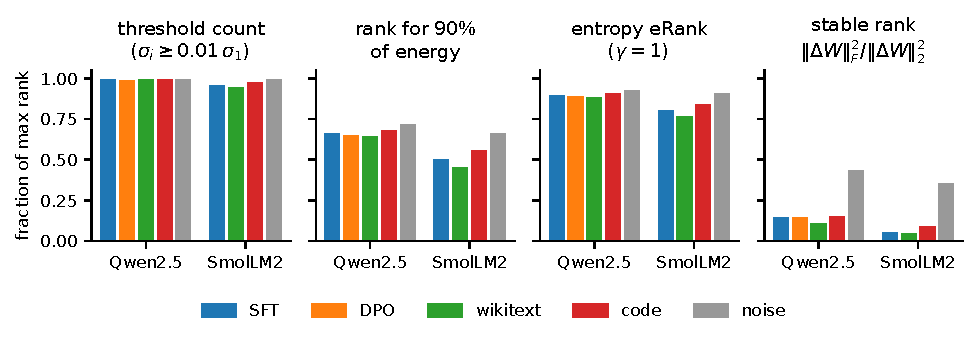
\includegraphics[width=\linewidth]{figures/metrics_vs_noise.pdf}
\end{center}
\caption{Four rank measures for our fine-tuning updates and for the random-init
pair of the same architecture (grey). The threshold count, the 90\%-energy rank
and the entropy effective rank put every update close to the noise value;
stable rank puts every update far below it. Means over 168 (Qwen2.5-0.5B) and
224 (SmolLM2-360M) matrices; DPO is measured against the SFT checkpoint.}
\label{fig:metrics}
\end{figure}

\begin{table}[t]
\caption{Rank measures as a fraction of the maximum rank, and the share of
energy in the top singular value. Last column: how many times lower the
update's stable rank is than the noise baseline's, with 95\% layer-bootstrap
intervals.}
\label{tab:metrics}
\begin{center}
\small
\begin{tabular}{llcccccc}
\toprule
 & & threshold & 90\% energy & eRank & stable & top-1 & noise / real \\
model & update & $\thresholdrank$ & $\energyrank$ & $\gamma=1$ & $\stablerank$ & energy & (stable) \\
\midrule
Qwen2.5-0.5B & SFT              & 0.991 & 0.660 & 0.893 & 0.145 & 5.1\% & 3.0 (2.7--3.4) \\
             & DPO (vs SFT)     & 0.990 & 0.652 & 0.891 & 0.144 & 5.5\% & 3.0 (2.7--3.4) \\
             & wikitext LM      & 0.990 & 0.643 & 0.881 & 0.110 & 6.9\% & 3.9 (3.5--4.5) \\
             & code LM          & 0.992 & 0.679 & 0.905 & 0.154 & 3.0\% & 2.8 (2.6--3.1) \\
             & random-init pair & 0.996 & 0.716 & 0.928 & 0.436 & 0.6\% & -- \\
\midrule
SmolLM2-360M & SFT              & 0.955 & 0.500 & 0.800 & 0.052 & 7.8\% & 6.9 (6.2--7.7) \\
             & wikitext LM      & 0.943 & 0.452 & 0.767 & 0.045 & 9.2\% & 7.9 (7.3--8.7) \\
             & code LM          & 0.976 & 0.559 & 0.841 & 0.089 & 4.7\% & 4.0 (3.6--4.5) \\
             & random-init pair & 0.996 & 0.659 & 0.908 & 0.354 & 0.5\% & -- \\
\bottomrule
\end{tabular}
\end{center}
\end{table}

Figure~\ref{fig:metrics} and Table~\ref{tab:metrics} compare the four measures
on our updates. The threshold count puts the Qwen updates at 99.0--99.2\% of
full rank against 99.6\% for the random-init pair, and the SmolLM2 updates at
94--98\% against 99.6\%. Read on its own, this says fine-tuning produces
updates of essentially full rank, which is how we first read it.
The 90\%-energy rank and the entropy effective rank move in the right
direction but by little: 0.64--0.68 against 0.72, and 0.88--0.91 against 0.93,
on Qwen. Stable rank instead puts every update 2.8--7.9$\times$ below the noise
baseline, with intervals far from 1.

The gap is consistent rather than random: the layer-bootstrap interval on the
noise-to-real ratio of the entropy effective rank stays above 1 for every run
(the closest is the code control, 1.023--1.030). So eRank does register the
structure, compressed into a few percent, where stable rank shows it as a
several-fold difference. Weighting $\sigma_i$ linearly inside an entropy lets
the long, flat part of the spectrum dominate.

The effect holds for every matrix type. For the Qwen SFT update, stable rank
is lower than noise by 3.7$\times$ for \texttt{q\_proj}, 5.1$\times$ for
\texttt{up\_proj} and 1.7$\times$ for \texttt{v\_proj}, the weakest case
(Appendix~\ref{app:pertype}).

\subsection{A noise-like tail and a few dominant directions}
\label{sec:headtail}

The measures disagree because the updates have two parts. The top of the
spectrum is far more concentrated than noise: the top singular value of the
Qwen SFT update holds 5.1\% of its energy against 0.6\% for the random pair,
the top 8 hold 12.0\% against 4.9\%, and the top 32 hold 26.0\% against
17.5\%. Below that, the spectrum decays slowly, much like a random matrix's.
Stable rank is dominated by the top, so it sees the concentration. The
threshold count and the energy rank count directions, most of which sit in
the tail, so they see a high-rank matrix. The entropy effective rank sits in
between.

Both statements, ``fine-tuning updates are high rank'' \citep{biderman2024lora}
and ``fine-tuning updates are concentrated'', are therefore true of the same
matrices. Which one a paper reports depends on the measure, and without a
noise baseline neither number says how much structure there is. The tail is
not negligible either: \S\ref{sec:cutoff} shows that deleting it hurts.

\subsection{Concentration is a property of fine-tuning, not of alignment}
\label{sec:controls}

\begin{table}[t]
\caption{Paired differences in stable rank (fraction of maximum rank) between
runs on the same base model, with 95\% layer-bootstrap intervals. Seed
differences compare runs with a different training seed and data sample.}
\label{tab:paired}
\begin{center}
\begin{tabular}{lcc}
\toprule
paired difference & Qwen2.5-0.5B & SmolLM2-360M \\
\midrule
code $-$ wikitext & $+0.044$ ($0.033$ to $0.054$) & $+0.044$ ($0.036$ to $0.052$) \\
SFT $-$ wikitext  & $+0.035$ ($0.025$ to $0.045$) & $+0.007$ ($0.003$ to $0.011$) \\
code $-$ SFT      & $+0.009$ ($-0.003$ to $0.020$) & $+0.037$ ($0.029$ to $0.045$) \\
\midrule
seed 43 $-$ seed 42, SFT      & $-0.003$ ($-0.010$ to $0.003$) & -- \\
seed 43 $-$ seed 42, wikitext & $-0.002$ ($-0.007$ to $0.002$) & -- \\
seed 43 $-$ seed 42, code     & $-0.002$ ($-0.008$ to $0.004$) & -- \\
\bottomrule
\end{tabular}
\end{center}
\end{table}

A concentrated SFT update is not evidence about alignment unless fine-tuning
on other data looks different. It does not. On Qwen, the wikitext control is
more concentrated than SFT (stable rank 0.110 against 0.145) and the code
control slightly less (0.154); on SmolLM2 all three are again well below noise
(Table~\ref{tab:metrics}). The updates also differ widely in size, with mean
Frobenius norms of 0.349 (wikitext), 0.280 (SFT), 0.127 (code) and 0.019 (DPO)
on Qwen, an 18-fold range, while their stable ranks stay between 0.110 and
0.154. Size and concentration are separate properties, which is why the
measures need to be scale-free.

Table~\ref{tab:paired} shows that the differences between tasks are real but
the ordering is not fixed. Repeating each Qwen run with a different seed and
data sample moves stable rank by at most 0.003, and every seed interval
contains zero. Wikitext is more concentrated than code on both models, by the
same 0.044. SFT, however, falls in a different place between them: on Qwen it
cannot be told apart from code, on SmolLM2 it sits close to wikitext. The
statement we can support is that the alignment update lies inside the range
spanned by the two non-alignment controls.

\subsection{Released base and instruct models up to 8B}
\label{sec:released}

\begin{figure}[t]
\begin{center}
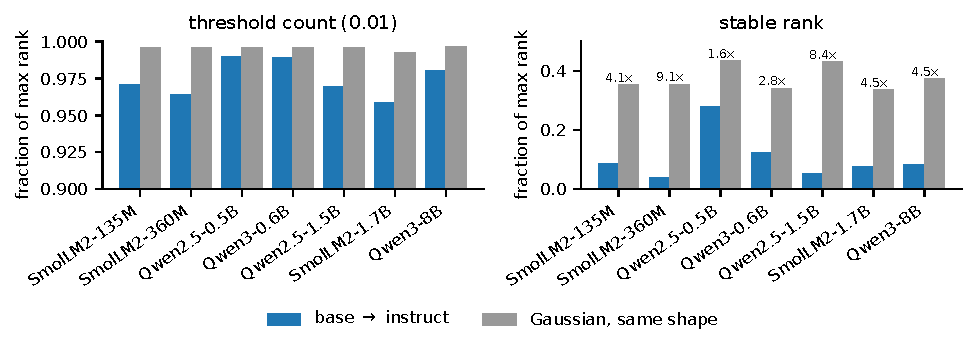
\includegraphics[width=\linewidth]{figures/released_pairs.pdf}
\end{center}
\caption{Official base $\to$ instruct updates (blue) against a Gaussian matrix of
the same shape (grey), ordered by model size. Left: the threshold count puts
every update within a few points of noise (note the axis starts at 0.9).
Right: stable rank puts every update 1.6--9.1$\times$ below noise.}
\label{fig:released}
\end{figure}

\begin{table}[t]
\caption{Released base/instruct pairs. Noise columns use a Gaussian matrix of
the same shape for every weight matrix. Last column: 95\% layer-bootstrap
interval on the ratio.}
\label{tab:released}
\begin{center}
\begin{tabular}{lccccc}
\toprule
pair & threshold & noise & stable rank & noise & noise / real \\
\midrule
SmolLM2-135M & 97.1\% & 99.6\% & 0.086 & 0.354 & 4.1 (3.5--5.0) \\
SmolLM2-360M & 96.4\% & 99.6\% & 0.039 & 0.356 & 9.1 (8.0--10.6) \\
Qwen2.5-0.5B & 99.0\% & 99.6\% & 0.280 & 0.434 & 1.6 (1.5--1.7) \\
Qwen3-0.6B   & 98.9\% & 99.6\% & 0.124 & 0.342 & 2.8 (2.6--3.0) \\
Qwen2.5-1.5B & 96.9\% & 99.6\% & 0.051 & 0.432 & 8.4 (7.7--9.2) \\
SmolLM2-1.7B & 95.9\% & 99.3\% & 0.075 & 0.336 & 4.5 (4.2--4.9) \\
Qwen3-8B     & 98.0\% & 99.6\% & 0.082 & 0.373 & 4.5 (4.2--5.0) \\
\bottomrule
\end{tabular}
\end{center}
\end{table}

Our fine-tunes are small, while released instruct models go through much
larger and mixed post-training. Figure~\ref{fig:released} and
Table~\ref{tab:released} show the same pattern on seven official pairs. The
threshold count reads 95.9--99.0\% for every update, within a few points of
noise; stable rank is 1.6--9.1$\times$ below noise for every one, including
Qwen3-8B at 4.5$\times$. The measurement problem is therefore not a property
of small runs, and it applies directly to the setting studied by prior work
on released models.

Qwen2.5-0.5B is the outlier, only 1.6$\times$ below noise and less
concentrated than our own SFT of the same base (0.280 against 0.145). We do
not know why. Nothing here says what the released post-training did, only that
its update is not noise-like.

\section{Case study: effective rank as evidence for superficial post-training}
\label{sec:timber}

\citet{wu2025timber} compare released base and instruct models (Llama~3 and
Qwen3) through the entropy effective rank of each weight matrix. They report
that $\entropyrank(W_{\text{base}})$ and $\entropyrank(W_{\text{instruct}})$
are nearly identical for every layer, read this as weight-level evidence that
post-training is superficial, and report $\entropyrank(\dW)$ at around 85\% of
full rank. They then edit instruct models by keeping the top
$K = \lceil \entropyrank(\dW) \rceil$ singular directions of $\dW$ and scaling
the rest by $\lambda \in [0, 1)$, which improves pass@$k$ on their benchmarks.
We test the measurement and the cutoff with the baselines of
\S\ref{sec:background}.

\paragraph{Reproduction.} On Qwen3-0.6B and Qwen3-8B, two of the pairs in
their study, we measure $\entropyrank(\dW)$ at 83\% of full rank for both,
consistent with their figure.

\subsection{An unchanged effective rank is what any small update produces}

\begin{figure}[t]
\begin{center}
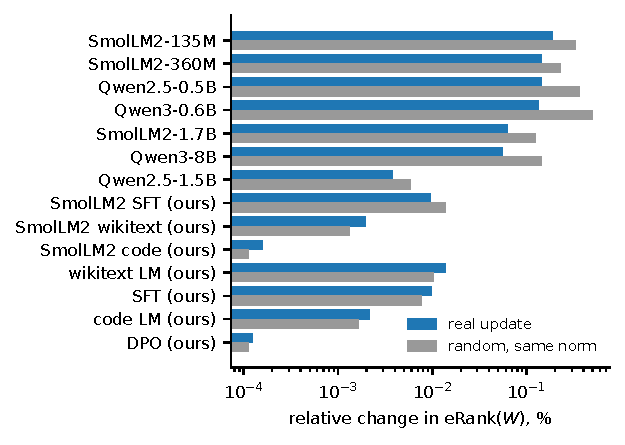
\includegraphics[width=0.62\linewidth]{figures/erank_perturbation.pdf}
\end{center}
\caption{Relative change in the entropy effective rank of the full weight
matrix $W$ caused by the real update (blue) and by a Gaussian perturbation
with the same Frobenius norm (grey), averaged over matrices. Log scale. Every
change, real or random, is below 0.5\%.}
\label{fig:erank}
\end{figure}

For every matrix we compare the change in $\entropyrank(W)$ caused by the real
update with the change caused by a random perturbation of the same norm
(Figure~\ref{fig:erank}; Table~\ref{tab:erankw} in the appendix). The update
is 0.05--1.4\% of $\|W\|_F$ for our runs and 1.2--12.6\% for the released
models. Across all fourteen cases the effective rank of $W$ moves by less than
0.5\%, and the random perturbation moves it by a similar amount: for Qwen3-8B,
0.06\% for the real update and 0.14\% for the random one; for our SFT run,
0.010\% and 0.008\%. This is the behaviour Weyl's inequality predicts, and it
means an unchanged effective rank of $W$ follows from the update being small.
It holds equally for our fine-tunes on Wikipedia and on code, so it cannot
distinguish superficial post-training from ordinary fine-tuning.

There is one detail in Timber's favour. On the released models the real
update moves the effective rank 1.5--4$\times$ less than a random one of the
same norm, so post-training does change $W$ in a structured way. That only
becomes visible with the random comparison, and it is a statement about
structure, not about superficiality.

\subsection{The effective rank of the update sits near the noise value}

On the update itself, $\entropyrank(\dW)$ is 0.79--0.90 of full rank for the
released pairs against 0.87--0.93 for Gaussian matrices of the same shapes, a
ratio of 1.03--1.14 (Qwen3-8B: 0.83 against 0.91). Stable rank separates the
same updates from noise by 1.6--9.1$\times$ (\S\ref{sec:released}). The
eRank-based cutoff of 83\% of full rank therefore sits close to where a random
matrix would put it.

\subsection{Does the cutoff matter?}
\label{sec:cutoff}

\begin{figure}[t]
\begin{center}
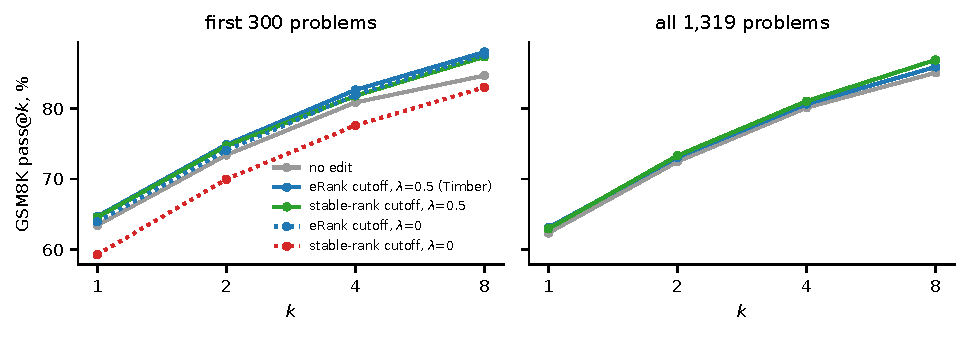
\includegraphics[width=\linewidth]{figures/cutoff_passk.pdf}
\end{center}
\caption{GSM8K pass@$k$ for Qwen3-0.6B (non-thinking mode) edited as in
\citet{wu2025timber}, with their eRank cutoff and with a stable-rank cutoff.
Left: the first 300 test problems, all five variants. Right: all 1{,}319
problems for the unedited model and the two $\lambda=0.5$ variants. Eight
samples per problem, the same sampling seed per problem for every variant.}
\label{fig:cutoff}
\end{figure}

\begin{table}[t]
\caption{Timber's edit on Qwen3-0.6B with two cutoffs, on all 1{,}319 GSM8K
test problems (8 samples each). ``Kept'' is the share of $\dW$'s energy left
unscaled. Differences from the unedited model are in points, with 95\% paired
bootstrap intervals over problems.}
\label{tab:cutoff}
\begin{center}
\small
\begin{tabular}{lccccc}
\toprule
variant & kept & pass@1 & pass@8 & $\Delta$ pass@1 & $\Delta$ pass@8 \\
\midrule
no edit                              & 100\%  & 62.3 & 85.1 & -- & -- \\
eRank cutoff, $\lambda=0.5$ (Timber) & 98.9\% & 63.1 & 85.9 & $+0.8$ ($-0.0$, $+1.6$) & $+0.8$ ($-0.6$, $+2.3$) \\
stable cutoff, $\lambda=0.5$         & 41.4\% & 62.9 & 86.9 & $+0.6$ ($-0.5$, $+1.7$) & $+1.8$ ($+0.2$, $+3.5$) \\
\bottomrule
\end{tabular}
\end{center}
\end{table}

On Qwen3-0.6B the eRank cutoff keeps 83\% of the directions and 98.9\% of the
update's energy, so Timber's edit changes about 1\% of the update. A cutoff at
$\lceil r \cdot \stablerank(\dW) \rceil$ keeps 12\% of the directions and
41\% of the energy. We apply the same edit with both cutoffs, at $\lambda = 0$
(their Timber-L) and $\lambda = 0.5$, and score pass@$k$ \citep{chen2021codex}
on GSM8K \citep{cobbe2021gsm8k} in non-thinking mode with the sampling
settings recommended for it (temperature 0.7, top-$p$ 0.8, top-$k$ 20).
\citet{wu2025timber} did not report GSM8K, so this is a test of the cutoff
rather than a reproduction of their table.

Three findings (Figure~\ref{fig:cutoff}, Table~\ref{tab:cutoff}):

\begin{itemize}
  \item \textbf{Removing the tail hurts.} On the first 300 problems, the
  stable-rank cutoff at $\lambda = 0$ lowers pass@1 by 4.2 points (interval
  $-6.9$ to $-1.4$), and the share of samples that reach a final answer falls
  from 96.5\% to 90.6\%. The noise-like 59\% of the update's energy matters to
  the model, which agrees with the finding of \citet{ping2024deltacome} that
  truncating $\dW$ to low rank degrades fine-tuned models.
  \item \textbf{Halving it does not.} At $\lambda = 0.5$ the two cutoffs give
  the same result. Directly compared on all 1{,}319 problems, the stable-rank
  variant differs from Timber's by $-0.2$ points of pass@1 ($-1.2$ to
  $+0.9$) and $+1.0$ of pass@8 ($-0.6$ to $+2.5$), although it scales about
  40$\times$ more of the update. The eRank boundary is not special.
  \item \textbf{The benefit is small on this benchmark.} On the first 300
  problems Timber's edit raised pass@8 by 3.3 points ($+0.3$ to $+6.3$), the
  pattern their paper reports. On the full set the gain is $+0.8$ ($-0.6$ to
  $+2.3$), and on the 1{,}019 problems outside the first 300 it is $+0.1$
  ($-1.6$ to $+1.7$). The only interval in Table~\ref{tab:cutoff} that clears
  zero, pass@8 for the stable-rank variant, does so by little among six
  comparisons, and we do not read anything into it.
\end{itemize}

None of this contradicts the gains \citet{wu2025timber} report on other
benchmarks, which we did not test. It does say that the effective rank of
$\dW$ is not what makes the edit work, and that pass@$k$ gains measured on a
few hundred problems can shrink substantially on the full set.

\section{Related work}
\label{sec:related}

\paragraph{Superficial alignment.} \citet{zhou2023lima} proposed that
alignment mostly selects a format the pretrained model already supports, and
\citet{lin2024urial} found that base and aligned models differ mainly on a
small set of stylistic tokens. \citet{wu2025timber} looked for weight-level
evidence through the effective rank of released models, which we examine in
\S\ref{sec:timber}. \citet{chaudhury2025alignment} locate the effect of
preference tuning in a few middle layers by activation patching, a causal
question about activations that our analysis of weights does not address.

\paragraph{Structure of fine-tuning updates.} \citet{aghajanyan2021intrinsic}
showed that fine-tuning can be carried out in a small random subspace, the
idea that LoRA \citep{hu2022lora} builds on, and \citet{ryu2023efficient}
store fine-tuned models as low-rank approximations of the weight residual.
\citet{biderman2024lora} measured full fine-tuning updates with the rank
needed for 90\% of the variance and found them 10--100$\times$ higher rank
than typical LoRA ranks; they also noted that adding small Gaussian noise to
$W$ leaves its spectrum similar, which is close in spirit to our same-norm
check, applied there to $W$ rather than as a control for a claim about
alignment. Our results agree with theirs and add the other half of the
picture: the same updates are also several times more concentrated than noise
at the top of the spectrum. \citet{shuttleworth2025lora} compare the singular
vectors of fine-tuned and pretrained $W$ and find that LoRA introduces
``intruder dimensions'' that full fine-tuning does not. Delta-CoMe
\citep{ping2024deltacome} compresses $\dW$ with more bits for the top singular
vectors, motivated by the same long-tailed spectrum, and finds that pure
low-rank truncation hurts. \citet{paul2026spectral} use stable rank among
other shape features of LoRA updates to tell training objectives apart. To
our knowledge none of these compares rank measures of $\dW$ against a noise
baseline matrix by matrix, or uses non-alignment fine-tunes as a control for
claims about alignment.

\paragraph{The measures.} Stable rank, also called numerical rank, comes from
\citet{rudelson2007sampling}, and the entropy effective rank from
\citet{roy2007effective}. Neither is new; the question here is only which of
them can tell a weight update from noise.

\section{Limitations}
\label{sec:limitations}

\begin{itemize}
  \item \textbf{Scale of our own training.} Our fine-tunes are 0.36B and 0.5B
  parameters with about two million tokens each. The measurement results
  hold on released models up to 8B, but we say nothing about how training
  itself behaves at that scale.
  \item \textbf{Behaviour on one model.} The evaluations, the LoRA sweep, DPO
  and the overlap analysis are all on Qwen2.5-0.5B and single-seed. SmolLM2
  replicates the spectral results only.
  \item \textbf{Released models are black boxes.} We do not know their
  post-training data or recipes, so they test the measurement but not any
  claim about alignment specifically.
  \item \textbf{Loss masking differs.} SFT computes loss on answer tokens only,
  the controls on every token. Tokens seen are matched; tokens trained on are
  not.
  \item \textbf{The cutoff test is narrow.} One model, one benchmark, one
  sampling mode. Gains reported by \citet{wu2025timber} on other benchmarks
  are untested here.
  \item \textbf{LoRA learning rates.} The lowest learning rate in the sweep
  won at every rank, so the rank-versus-GSM8K trend may partly reflect
  under-tuned learning rates.
\end{itemize}

\section{Conclusion}
\label{sec:conclusion}

Measures that count directions, whether by threshold, by energy share or by
entropy, describe fine-tuning updates as nearly full rank and put them within
a few percent of random matrices of the same shape. Stable rank shows the same
updates to be several times more concentrated than noise. Both descriptions
are accurate, because the updates combine a noise-like tail with a few
dominant directions, and the tail matters to the model. The practical lesson
is simple: a rank measure of a weight update means little without the same
measure on a matrix with no structure, and a claim about alignment needs a
fine-tune without alignment content as its control. With both in place, the
concentration of the update turns out to be a property of fine-tuning in
general, and an unchanged effective rank after post-training turns out to be
what any small update produces.

\subsubsection*{Broader Impact Statement}
This work is about measurement methodology for analysing fine-tuned language
models. It does not introduce new capabilities or training methods. Its main
practical consequence is caution about reading weight-space statistics as
evidence that alignment is shallow or deep; claims of either kind can affect
how much trust is placed in alignment training, and they should rest on
measurements with proper baselines.

% Reproducibility: code, configs, exact training rows, result CSVs and the
% saved singular-value spectra will be released with the camera-ready version
% (kept out of the anonymous submission).


\bibliography{main}
\bibliographystyle{tmlr}

\appendix
\section{Training details}
\label{app:training}

\begin{table}[h]
\caption{Settings shared by all our fine-tunes. Each run trains on the same
number of tokens as the SFT run of the same model, counted after truncation.}
\label{tab:hparams}
\begin{center}
\small
\begin{tabular}{ll}
\toprule
setting & value \\
\midrule
weights / compute precision & fp32 master weights, bf16 autocast \\
optimizer                   & 8-bit AdamW, learning rate $2\times10^{-5}$, no weight decay \\
schedule                    & cosine, 3\% warmup, 3 epochs, gradient clipping at 1.0 \\
batch                       & 1 sequence $\times$ 16 accumulation steps \\
sequence length             & 512 tokens \\
embeddings                  & frozen (tied with the output head; not analysed) \\
memory                      & gradient checkpointing, one 6\,GB GPU \\
check after training        & at most $1.1\times10^{-5}$ of attention/MLP weights unchanged \\
\midrule
SFT data                    & 10k examples of Alpaca-cleaned, loss on answers only \\
wikitext / code data        & wikitext-103 / CodeParrot (Python), plain LM loss \\
shuffled-words data         & wikitext documents, word order shuffled within each document \\
training tokens             & Qwen: 1.71--1.75M; SmolLM2: 1.87--1.91M \\
\bottomrule
\end{tabular}
\end{center}
\end{table}

Training a run took 1.3--3.7 hours. The base tokenizer of SmolLM2-360M has no
chat template, so SFT borrows the one from SmolLM2-360M-Instruct. Second seeds
change both the training seed and the data sample. Every run records its exact
training rows, token count and the fraction of unchanged weights.

\section{Threshold sensitivity and the noise baseline}
\label{app:sensitivity}

\begin{table}[h]
\caption{The threshold count at three cut-offs. At $0.01\,\sigma_1$ every
update looks almost like noise; at $0.1\,\sigma_1$ the gap is large. The verdict
depends on an arbitrary choice.}
\label{tab:threshold}
\begin{center}
\small
\begin{tabular}{llccc}
\toprule
model & matrix & $0.01\,\sigma_1$ & $0.05\,\sigma_1$ & $0.1\,\sigma_1$ \\
\midrule
Qwen2.5-0.5B & SFT update            & 0.973 & 0.889 & 0.787 \\
             & wikitext update       & 0.972 & 0.886 & 0.775 \\
             & code update           & 0.975 & 0.895 & 0.799 \\
             & shuffled-words update & 0.941 & 0.752 & 0.530 \\
             & noise                 & 0.996 & 0.982 & 0.964 \\
             & pretrained $W$        & 0.976 & 0.913 & 0.851 \\
\midrule
SmolLM2-360M & SFT update            & 0.951 & 0.757 & 0.458 \\
             & wikitext update       & 0.948 & 0.701 & 0.386 \\
             & code update           & 0.963 & 0.803 & 0.534 \\
             & shuffled-words update & 0.863 & 0.384 & 0.151 \\
             & noise                 & 0.996 & 0.982 & 0.964 \\
             & pretrained $W$        & 0.982 & 0.926 & 0.857 \\
\bottomrule
\end{tabular}
\end{center}
\end{table}

\begin{table}[h]
\caption{Stable rank of the random-init pair against the prediction
$mn/(\sqrt{m}+\sqrt{n})^2/r$ for a Gaussian matrix of the same shape,
Qwen2.5-0.5B, mean over layers.}
\label{tab:mp}
\begin{center}
\small
\begin{tabular}{lccc}
\toprule
matrix & shape & predicted & random-init pair \\
\midrule
\texttt{q}, \texttt{o} & $896 \times 896$  & 0.250 & 0.252, 0.251 \\
\texttt{k}, \texttt{v} & $128 \times 896$  & 0.527 & 0.536, 0.535 \\
\texttt{gate}, \texttt{up} & $4864 \times 896$ & 0.490 & 0.492, 0.492 \\
\texttt{down} & $896 \times 4864$ & 0.490 & 0.493 \\
\bottomrule
\end{tabular}
\end{center}
\end{table}

\section{Stable rank by matrix type}
\label{app:pertype}

\begin{table}[h]
\caption{Stable rank (fraction of maximum rank) by matrix type, Qwen2.5-0.5B.}
\label{tab:pertype}
\begin{center}
\small
\begin{tabular}{lccccccc}
\toprule
 & \texttt{q} & \texttt{k} & \texttt{v} & \texttt{o} & \texttt{gate} & \texttt{up} & \texttt{down} \\
\midrule
SFT update            & 0.032 & 0.064 & 0.251 & 0.057 & 0.064 & 0.072 & 0.139 \\
wikitext update       & 0.031 & 0.072 & 0.227 & 0.057 & 0.065 & 0.085 & 0.112 \\
code update           & 0.031 & 0.070 & 0.243 & 0.058 & 0.057 & 0.073 & 0.127 \\
shuffled-words update & 0.011 & 0.043 & 0.124 & 0.021 & 0.023 & 0.026 & 0.048 \\
noise                 & 0.252 & 0.536 & 0.535 & 0.251 & 0.492 & 0.492 & 0.493 \\
pretrained $W$        & 0.058 & 0.212 & 0.453 & 0.078 & 0.071 & 0.242 & 0.135 \\
\bottomrule
\end{tabular}
\end{center}
\end{table}

Every matrix type of every update is far below noise. The SFT, wikitext and
code updates agree closely in every column; the shuffled-words update is the
most concentrated in every column.

\section{The shuffled-words update}
\label{app:shuffled}

\begin{table}[h]
\caption{Stable rank by quarter of the network.}
\label{tab:shuffled}
\begin{center}
\small
\begin{tabular}{llcccc}
\toprule
model & update & first quarter & second & third & last quarter \\
\midrule
Qwen2.5-0.5B & SFT            & 0.094 & 0.099 & 0.103 & 0.091 \\
             & wikitext       & 0.086 & 0.100 & 0.104 & 0.080 \\
             & code           & 0.091 & 0.097 & 0.104 & 0.085 \\
             & shuffled words & 0.055 & 0.039 & 0.034 & 0.042 \\
\midrule
SmolLM2-360M & SFT            & 0.023 & 0.027 & 0.029 & 0.021 \\
             & wikitext       & 0.019 & 0.024 & 0.023 & 0.015 \\
             & code           & 0.030 & 0.038 & 0.043 & 0.027 \\
             & shuffled words & 0.013 & 0.010 & 0.007 & 0.007 \\
\bottomrule
\end{tabular}
\end{center}
\end{table}

To test whether the shuffled-words update mainly shifts the output towards
frequent tokens, we take the top left singular vector of each layer's
\texttt{down\_proj} update on Qwen, map it to the vocabulary through the final
norm and the tied unembedding, and correlate that logit shift with the log
frequency of each token in the run's training data, against 50 random
directions. In layers 18--22 the correlation is 0.32--0.39 for shuffled words,
above the random 95th percentile (about 0.19), while the wikitext run, trained
on the same words in their normal order, stays at 0.00--0.13. In the first two
thirds of the network the shuffled-words update shows no such alignment, so
frequency explains only part of its concentration.

\section{Released pairs: more measures}
\label{app:released}

\begin{table}[h]
\caption{Participation ratio of each released update against a Gaussian matrix
of the same shape, the number of singular values above the largest one a
Gaussian matrix of the same shape and size would have (mean per matrix), and
the share of directions above the simulated bf16 rounding floor.}
\label{tab:released_more}
\begin{center}
\small
\begin{tabular}{lcccc}
\toprule
update & particip. & noise & above noise edge & above rounding floor \\
\midrule
SmolLM2-135M instruct & 0.321 & 0.667 & 30  & 96\% \\
SmolLM2-360M instruct & 0.239 & 0.668 & 46  & 95\% \\
Qwen2.5-0.5B instruct & 0.657 & 0.755 & 22  & 97\% \\
Qwen3-0.6B            & 0.442 & 0.654 & 72  & 99\% \\
Qwen2.5-1.5B instruct & 0.299 & 0.753 & 100 & 78\% \\
SmolLM2-1.7B instruct & 0.375 & 0.629 & 140 & 91\% \\
Qwen3-8B              & 0.405 & 0.693 & 243 & 97\% \\
OLMo 2 1B: base $\to$ SFT & 0.435 & 0.629 & 85  & -- \\
OLMo 2 1B: SFT $\to$ DPO  & 0.116 & 0.629 & 114 & 13\% \\
OLMo 2 1B: DPO $\to$ RL   & 0.127 & 0.629 & 99  & 3\% \\
Qwen2.5-Coder-0.5B    & 0.545 & 0.755 & 44  & 100\% \\
Qwen2.5-Math-1.5B     & 0.611 & 0.753 & 61  & 100\% \\
Qwen2.5-Coder-1.5B    & 0.585 & 0.753 & 66  & 100\% \\
\bottomrule
\end{tabular}
\end{center}
\end{table}

Qwen2.5-0.5B is the least concentrated instruct release on every measure, and
less concentrated than our own SFT of the same base; we do not know why.

\section{Edit experiment details}
\label{app:cutoff}

The prompt is the GSM8K question followed by ``Please reason step by step, and
put your final answer within \verb|\boxed{}|.'', in Qwen3's chat template with
thinking turned off, sampled at temperature 0.7, top-$p$ 0.8 and top-$k$ 20 for
up to 512 new tokens. The answer is the last \verb|\boxed{}| expression, or the
last number if there is none. The edit is applied to every attention and MLP
projection in fp32 and the model then runs in bf16, which distorts the edit by
25\% of its size for Timber's tail edit, 4\% for the stable-rank tail edit and
6\% for uniform scaling. pass@$k$ uses the unbiased estimator of
\citet{chen2021codex} with $n=8$.

\begin{table}[h]
\caption{All edit variants on the first 300 GSM8K test problems. Differences
from the unedited model in points, with 95\% paired bootstrap intervals.
``Answered'' is the share of samples with a final boxed answer.}
\label{tab:cutoff300}
\begin{center}
\small
\begin{tabular}{lccccc}
\toprule
edit & pass@1 & pass@8 & answered & $\Delta$ pass@1 & $\Delta$ pass@8 \\
\midrule
none                                  & 63.4 & 84.7 & 96.5\% & -- & -- \\
tail $\times 0$, eRank cutoff         & 63.9 & 87.7 & 96.7\% & $+0.5$ ($-1.3$, $+2.3$) & $+3.0$ ($-0.3$, $+6.3$) \\
tail $\times 0.5$, eRank cutoff       & 64.7 & 88.0 & 96.8\% & $+1.3$ ($-0.5$, $+3.0$) & $+3.3$ ($+0.3$, $+6.3$) \\
tail $\times 0$, stable-rank cutoff   & 59.3 & 83.0 & 90.6\% & $-4.2$ ($-6.9$, $-1.4$) & $-1.7$ ($-5.7$, $+2.3$) \\
tail $\times 0.5$, stable-rank cutoff & 64.5 & 87.3 & 95.1\% & $+1.1$ ($-1.2$, $+3.4$) & $+2.7$ ($-1.0$, $+6.3$) \\
whole update $\times 0.75$            & 66.0 & 88.7 & 96.0\% & $+2.6$ ($+0.5$, $+4.8$) & $+4.0$ ($+1.3$, $+7.0$) \\
\bottomrule
\end{tabular}
\end{center}
\end{table}


\end{document}
